\documentclass{standalone}
\usepackage{tikz}
\begin{document}
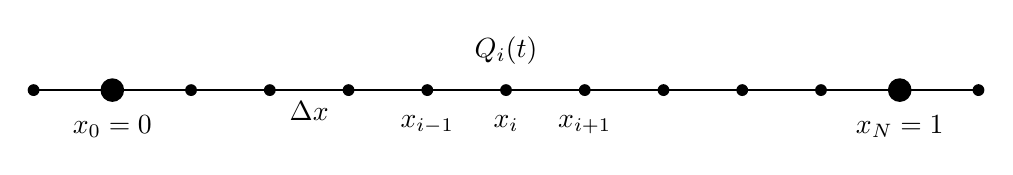
\begin{tikzpicture}
\draw [thick] (-1,0) -- (11,0);
\foreach \x in {-1,...,11}{
    \fill (\x,0) circle(.075);
}
\fill (0,0) circle(.15);
\fill (10,0) circle(.15);

\node[anchor=north] at (0,-0.2) {$x_{0} = 0$};
\node[anchor=north] at (4,-0.2) {$x_{i-1}$};
\node[anchor=north] at (5,-0.2) {$x_{i}$};
\node[anchor=north] at (6,-0.2) {$x_{i+1}$};
\node[anchor=north] at (10,-0.2) {$x_N = 1$};
\node[anchor=south] at (5,0.2) {$Q_i(t)$};
\node[anchor=north] at (2.5,-0.025) {$\Delta x$};
\end{tikzpicture}
\end{document}